% Options for packages loaded elsewhere
\PassOptionsToPackage{unicode}{hyperref}
\PassOptionsToPackage{hyphens}{url}
%
\documentclass[
]{article}
\usepackage{amsmath,amssymb}
\usepackage{iftex}
\ifPDFTeX
  \usepackage[T1]{fontenc}
  \usepackage[utf8]{inputenc}
  \usepackage{textcomp} % provide euro and other symbols
\else % if luatex or xetex
  \usepackage{unicode-math} % this also loads fontspec
  \defaultfontfeatures{Scale=MatchLowercase}
  \defaultfontfeatures[\rmfamily]{Ligatures=TeX,Scale=1}
\fi
\usepackage{lmodern}
\ifPDFTeX\else
  % xetex/luatex font selection
\fi
% Use upquote if available, for straight quotes in verbatim environments
\IfFileExists{upquote.sty}{\usepackage{upquote}}{}
\IfFileExists{microtype.sty}{% use microtype if available
  \usepackage[]{microtype}
  \UseMicrotypeSet[protrusion]{basicmath} % disable protrusion for tt fonts
}{}
\makeatletter
\@ifundefined{KOMAClassName}{% if non-KOMA class
  \IfFileExists{parskip.sty}{%
    \usepackage{parskip}
  }{% else
    \setlength{\parindent}{0pt}
    \setlength{\parskip}{6pt plus 2pt minus 1pt}}
}{% if KOMA class
  \KOMAoptions{parskip=half}}
\makeatother
\usepackage{xcolor}
\usepackage[margin=1in]{geometry}
\usepackage{color}
\usepackage{fancyvrb}
\newcommand{\VerbBar}{|}
\newcommand{\VERB}{\Verb[commandchars=\\\{\}]}
\DefineVerbatimEnvironment{Highlighting}{Verbatim}{commandchars=\\\{\}}
% Add ',fontsize=\small' for more characters per line
\usepackage{framed}
\definecolor{shadecolor}{RGB}{248,248,248}
\newenvironment{Shaded}{\begin{snugshade}}{\end{snugshade}}
\newcommand{\AlertTok}[1]{\textcolor[rgb]{0.94,0.16,0.16}{#1}}
\newcommand{\AnnotationTok}[1]{\textcolor[rgb]{0.56,0.35,0.01}{\textbf{\textit{#1}}}}
\newcommand{\AttributeTok}[1]{\textcolor[rgb]{0.13,0.29,0.53}{#1}}
\newcommand{\BaseNTok}[1]{\textcolor[rgb]{0.00,0.00,0.81}{#1}}
\newcommand{\BuiltInTok}[1]{#1}
\newcommand{\CharTok}[1]{\textcolor[rgb]{0.31,0.60,0.02}{#1}}
\newcommand{\CommentTok}[1]{\textcolor[rgb]{0.56,0.35,0.01}{\textit{#1}}}
\newcommand{\CommentVarTok}[1]{\textcolor[rgb]{0.56,0.35,0.01}{\textbf{\textit{#1}}}}
\newcommand{\ConstantTok}[1]{\textcolor[rgb]{0.56,0.35,0.01}{#1}}
\newcommand{\ControlFlowTok}[1]{\textcolor[rgb]{0.13,0.29,0.53}{\textbf{#1}}}
\newcommand{\DataTypeTok}[1]{\textcolor[rgb]{0.13,0.29,0.53}{#1}}
\newcommand{\DecValTok}[1]{\textcolor[rgb]{0.00,0.00,0.81}{#1}}
\newcommand{\DocumentationTok}[1]{\textcolor[rgb]{0.56,0.35,0.01}{\textbf{\textit{#1}}}}
\newcommand{\ErrorTok}[1]{\textcolor[rgb]{0.64,0.00,0.00}{\textbf{#1}}}
\newcommand{\ExtensionTok}[1]{#1}
\newcommand{\FloatTok}[1]{\textcolor[rgb]{0.00,0.00,0.81}{#1}}
\newcommand{\FunctionTok}[1]{\textcolor[rgb]{0.13,0.29,0.53}{\textbf{#1}}}
\newcommand{\ImportTok}[1]{#1}
\newcommand{\InformationTok}[1]{\textcolor[rgb]{0.56,0.35,0.01}{\textbf{\textit{#1}}}}
\newcommand{\KeywordTok}[1]{\textcolor[rgb]{0.13,0.29,0.53}{\textbf{#1}}}
\newcommand{\NormalTok}[1]{#1}
\newcommand{\OperatorTok}[1]{\textcolor[rgb]{0.81,0.36,0.00}{\textbf{#1}}}
\newcommand{\OtherTok}[1]{\textcolor[rgb]{0.56,0.35,0.01}{#1}}
\newcommand{\PreprocessorTok}[1]{\textcolor[rgb]{0.56,0.35,0.01}{\textit{#1}}}
\newcommand{\RegionMarkerTok}[1]{#1}
\newcommand{\SpecialCharTok}[1]{\textcolor[rgb]{0.81,0.36,0.00}{\textbf{#1}}}
\newcommand{\SpecialStringTok}[1]{\textcolor[rgb]{0.31,0.60,0.02}{#1}}
\newcommand{\StringTok}[1]{\textcolor[rgb]{0.31,0.60,0.02}{#1}}
\newcommand{\VariableTok}[1]{\textcolor[rgb]{0.00,0.00,0.00}{#1}}
\newcommand{\VerbatimStringTok}[1]{\textcolor[rgb]{0.31,0.60,0.02}{#1}}
\newcommand{\WarningTok}[1]{\textcolor[rgb]{0.56,0.35,0.01}{\textbf{\textit{#1}}}}
\usepackage{graphicx}
\makeatletter
\def\maxwidth{\ifdim\Gin@nat@width>\linewidth\linewidth\else\Gin@nat@width\fi}
\def\maxheight{\ifdim\Gin@nat@height>\textheight\textheight\else\Gin@nat@height\fi}
\makeatother
% Scale images if necessary, so that they will not overflow the page
% margins by default, and it is still possible to overwrite the defaults
% using explicit options in \includegraphics[width, height, ...]{}
\setkeys{Gin}{width=\maxwidth,height=\maxheight,keepaspectratio}
% Set default figure placement to htbp
\makeatletter
\def\fps@figure{htbp}
\makeatother
\setlength{\emergencystretch}{3em} % prevent overfull lines
\providecommand{\tightlist}{%
  \setlength{\itemsep}{0pt}\setlength{\parskip}{0pt}}
\setcounter{secnumdepth}{-\maxdimen} % remove section numbering
\usepackage{caption}
\usepackage{booktabs}
\usepackage{makecell}
\usepackage{longtable}
\usepackage{array}
\usepackage{multirow}
\usepackage{wrapfig}
\usepackage{float}
\usepackage{colortbl}
\usepackage{pdflscape}
\usepackage{tabu}
\usepackage{threeparttable}
\usepackage{threeparttablex}
\usepackage[normalem]{ulem}
\usepackage{makecell}
\usepackage{xcolor}
\floatplacement{figure}{H}
\usepackage{booktabs}
\usepackage{longtable}
\usepackage{array}
\usepackage{multirow}
\usepackage{wrapfig}
\usepackage{float}
\usepackage{colortbl}
\usepackage{pdflscape}
\usepackage{tabu}
\usepackage{threeparttable}
\usepackage{threeparttablex}
\usepackage[normalem]{ulem}
\usepackage{makecell}
\usepackage{xcolor}
\ifLuaTeX
  \usepackage{selnolig}  % disable illegal ligatures
\fi
\usepackage{bookmark}
\IfFileExists{xurl.sty}{\usepackage{xurl}}{} % add URL line breaks if available
\urlstyle{same}
\hypersetup{
  pdftitle={heart\_disease\_ms},
  pdfauthor={Walter Guillioli},
  hidelinks,
  pdfcreator={LaTeX via pandoc}}

\title{heart\_disease\_ms}
\author{Walter Guillioli}
\date{04 September, 2024}

\begin{document}
\maketitle

\begin{Shaded}
\begin{Highlighting}[]
\CommentTok{\#$ disease \textless{}int\textgreater{} 2, 1, 2, 1, 1, 1, 2, 2, 2, 2, 1, 1, 1, 2, 1, 1, 2, 2, 1, 1, ...}
\CommentTok{\# Absence (1) or presence (2) of heart disease}

\NormalTok{d }\SpecialCharTok{\%\textgreater{}\%}
  \FunctionTok{group\_by}\NormalTok{(disease) }\SpecialCharTok{\%\textgreater{}\%}
  \FunctionTok{tally}\NormalTok{() }\SpecialCharTok{\%\textgreater{}\%}
  \FunctionTok{mutate}\NormalTok{(}\AttributeTok{p =}\NormalTok{ n}\SpecialCharTok{/}\FunctionTok{sum}\NormalTok{(n)) }\CommentTok{\#1 56\%, 2 44\%}
\end{Highlighting}
\end{Shaded}

\begin{verbatim}
## # A tibble: 2 x 3
##   disease     n     p
##     <int> <int> <dbl>
## 1       1   150 0.556
## 2       2   120 0.444
\end{verbatim}

\begin{Shaded}
\begin{Highlighting}[]
\NormalTok{d }\OtherTok{\textless{}{-}}\NormalTok{ d }\SpecialCharTok{\%\textgreater{}\%}
  \FunctionTok{mutate}\NormalTok{(}\AttributeTok{disease\_fct =} \FunctionTok{case\_match}\NormalTok{(d}\SpecialCharTok{$}\NormalTok{disease, }\DecValTok{1} \SpecialCharTok{\textasciitilde{}} \StringTok{"N"}\NormalTok{, }\DecValTok{2} \SpecialCharTok{\textasciitilde{}} \StringTok{"Y"}\NormalTok{, }\AttributeTok{.default =} \ConstantTok{NA}\NormalTok{)) }\SpecialCharTok{\%\textgreater{}\%}
  \FunctionTok{mutate}\NormalTok{(}\AttributeTok{disease\_fct=} \FunctionTok{as.factor}\NormalTok{(disease\_fct)) }\SpecialCharTok{\%\textgreater{}\%}
  \FunctionTok{select}\NormalTok{(}\SpecialCharTok{{-}}\NormalTok{disease)}
\end{Highlighting}
\end{Shaded}

\begin{Shaded}
\begin{Highlighting}[]
\CommentTok{\# For numeric, see distribution, cap or convert scale to normalize, see}
\CommentTok{\# potential of prediction for disease (remove if none), bin/flag if appropriate}

\CommentTok{\# For discrete, see potential of prediction and bin as needed to help ML}

\CommentTok{\#$ age     \textless{}dbl\textgreater{} 70, 67, 57, 64, 74, 65, 56, 59, 60, 63, 59, 53, 44, 61, 57, …}
\FunctionTok{get\_percentiles}\NormalTok{(d}\SpecialCharTok{$}\NormalTok{age) }\CommentTok{\#29 to 77}
\end{Highlighting}
\end{Shaded}

\begin{verbatim}
##    0%    1%    5%   10%   25%   50%   75%   90%   95%   99%  100% 
## 29.00 34.69 40.00 42.00 48.00 55.00 61.00 66.00 68.00 71.93 77.00
\end{verbatim}

\begin{Shaded}
\begin{Highlighting}[]
\FunctionTok{hist}\NormalTok{(d}\SpecialCharTok{$}\NormalTok{age)}
\end{Highlighting}
\end{Shaded}

\begin{center}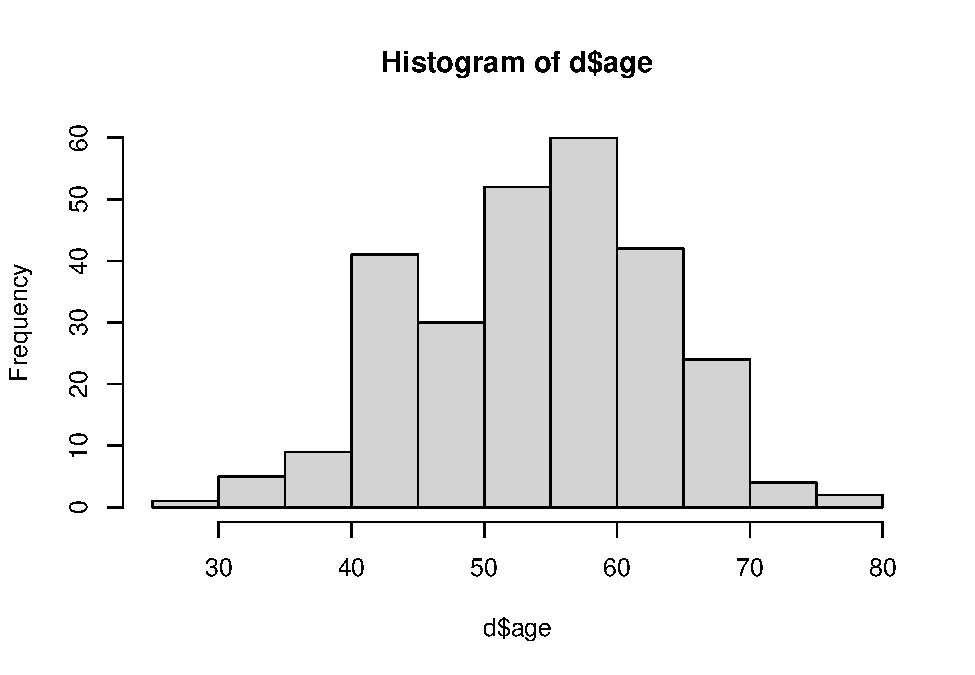
\includegraphics[width=0.8\linewidth]{heart_disease_ms_files/figure-latex/eda_x-1} \end{center}

\begin{Shaded}
\begin{Highlighting}[]
\FunctionTok{boxplot}\NormalTok{(age }\SpecialCharTok{\textasciitilde{}}\NormalTok{ disease\_fct, d, }\AttributeTok{horizontal =} \ConstantTok{TRUE}\NormalTok{) }\CommentTok{\#some power of prediction }
\end{Highlighting}
\end{Shaded}

\begin{center}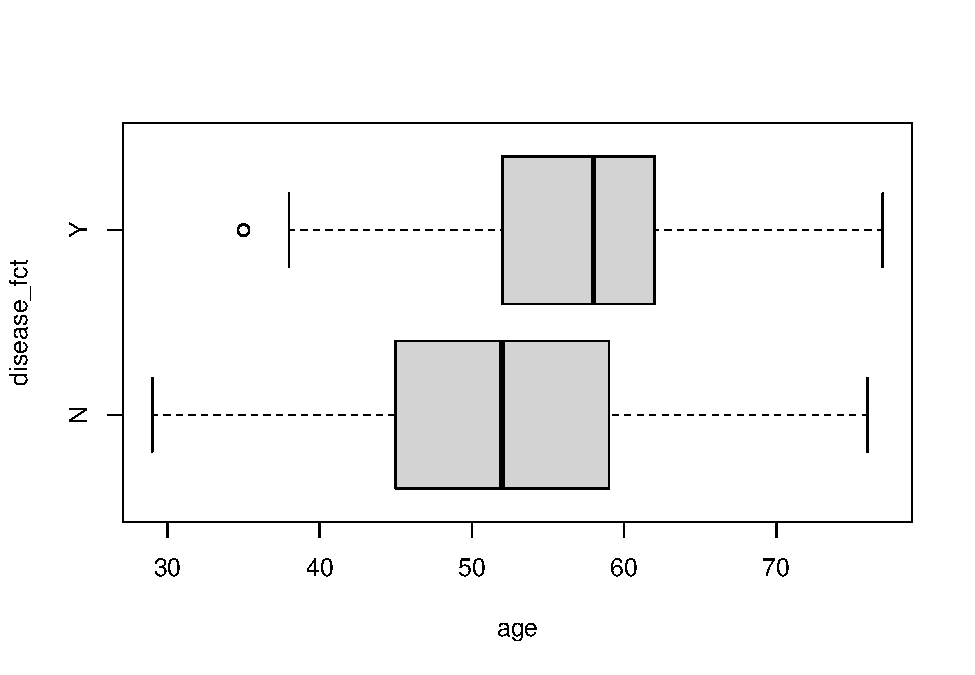
\includegraphics[width=0.8\linewidth]{heart_disease_ms_files/figure-latex/eda_x-2} \end{center}

\begin{Shaded}
\begin{Highlighting}[]
\NormalTok{d }\SpecialCharTok{\%\textgreater{}\%}
  \FunctionTok{group\_by}\NormalTok{(disease\_fct) }\SpecialCharTok{\%\textgreater{}\%}
  \FunctionTok{summarise}\NormalTok{(}\AttributeTok{median =} \FunctionTok{median}\NormalTok{(age),}
            \AttributeTok{p25 =} \FunctionTok{quantile}\NormalTok{(age, }\AttributeTok{p =} \FloatTok{0.25}\NormalTok{),}
            \AttributeTok{p75 =} \FunctionTok{quantile}\NormalTok{(age, }\AttributeTok{p =} \FloatTok{0.75}\NormalTok{)) }
\end{Highlighting}
\end{Shaded}

\begin{verbatim}
## # A tibble: 2 x 4
##   disease_fct median   p25   p75
##   <fct>        <dbl> <dbl> <dbl>
## 1 N               52    45    59
## 2 Y               58    52    62
\end{verbatim}

\begin{Shaded}
\begin{Highlighting}[]
\CommentTok{\#$ sex     \textless{}dbl\textgreater{} 1, 0, 1, 1, 0, 1, 1, 1, 1, 0, 1, 1, 1, 1, 0, 0, 1, 1, 1, 1, …}
\CommentTok{\# 0: female, 1: male}
\NormalTok{d }\OtherTok{\textless{}{-}}\NormalTok{ d }\SpecialCharTok{\%\textgreater{}\%}
  \FunctionTok{mutate}\NormalTok{(}\AttributeTok{sex\_fct =} \FunctionTok{as.factor}\NormalTok{(}\FunctionTok{recode}\NormalTok{(d}\SpecialCharTok{$}\NormalTok{sex, }\StringTok{\textquotesingle{}0\textquotesingle{}} \OtherTok{=} \StringTok{"F"}\NormalTok{, }\StringTok{\textquotesingle{}1\textquotesingle{}} \OtherTok{=} \StringTok{"M"}\NormalTok{))) }

\NormalTok{d }\SpecialCharTok{\%\textgreater{}\%}
  \FunctionTok{group\_by}\NormalTok{(sex\_fct) }\SpecialCharTok{\%\textgreater{}\%}
  \FunctionTok{tally}\NormalTok{() }\SpecialCharTok{\%\textgreater{}\%}
  \FunctionTok{mutate}\NormalTok{(}\AttributeTok{p=}\NormalTok{n}\SpecialCharTok{/}\FunctionTok{sum}\NormalTok{(n)) }\CommentTok{\#68\%M, 32\%F}
\end{Highlighting}
\end{Shaded}

\begin{verbatim}
## # A tibble: 2 x 3
##   sex_fct     n     p
##   <fct>   <int> <dbl>
## 1 F          87 0.322
## 2 M         183 0.678
\end{verbatim}

\begin{Shaded}
\begin{Highlighting}[]
\NormalTok{(t }\OtherTok{\textless{}{-}} \FunctionTok{table}\NormalTok{(d}\SpecialCharTok{$}\NormalTok{sex\_fct, d}\SpecialCharTok{$}\NormalTok{disease\_fct))}
\end{Highlighting}
\end{Shaded}

\begin{verbatim}
##    
##       N   Y
##   F  67  20
##   M  83 100
\end{verbatim}

\begin{Shaded}
\begin{Highlighting}[]
\FunctionTok{round}\NormalTok{(}\FunctionTok{prop.table}\NormalTok{(t, }\AttributeTok{margin =} \DecValTok{2}\NormalTok{), }\DecValTok{2}\NormalTok{) }\CommentTok{\#higher \% of males get Y, so has power}
\end{Highlighting}
\end{Shaded}

\begin{verbatim}
##    
##        N    Y
##   F 0.45 0.17
##   M 0.55 0.83
\end{verbatim}

\begin{Shaded}
\begin{Highlighting}[]
\CommentTok{\#$ pain    \textless{}dbl\textgreater{} 4, 3, 2, 4, 2, 4, 3, 4, 4, 4, 4, 4, 3, 1, 4, 4, 4, 4, 1, 1, 4 …}
\NormalTok{(t }\OtherTok{\textless{}{-}} \FunctionTok{table}\NormalTok{(d}\SpecialCharTok{$}\NormalTok{pain, d}\SpecialCharTok{$}\NormalTok{disease\_fct))}
\end{Highlighting}
\end{Shaded}

\begin{verbatim}
##    
##      N  Y
##   1 15  5
##   2 35  7
##   3 62 17
##   4 38 91
\end{verbatim}

\begin{Shaded}
\begin{Highlighting}[]
\FunctionTok{round}\NormalTok{(}\FunctionTok{prop.table}\NormalTok{(t, }\AttributeTok{margin =} \DecValTok{2}\NormalTok{), }\DecValTok{2}\NormalTok{) }\CommentTok{\#good power 4 vs others, 1{-}3 low count}
\end{Highlighting}
\end{Shaded}

\begin{verbatim}
##    
##        N    Y
##   1 0.10 0.04
##   2 0.23 0.06
##   3 0.41 0.14
##   4 0.25 0.76
\end{verbatim}

\begin{Shaded}
\begin{Highlighting}[]
\NormalTok{d }\OtherTok{\textless{}{-}}\NormalTok{ d }\SpecialCharTok{\%\textgreater{}\%}
  \FunctionTok{mutate}\NormalTok{(}\AttributeTok{pain\_fct =} \FunctionTok{as.factor}\NormalTok{(}\FunctionTok{ifelse}\NormalTok{(pain }\SpecialCharTok{==} \DecValTok{4}\NormalTok{, }\StringTok{"4"}\NormalTok{, }\StringTok{"1{-}3"}\NormalTok{))) }

\CommentTok{\#$ sugar   \textless{}dbl\textgreater{} 0, 0, 0, 0, 0, 0, 1, 0, 0, 0, 0, 0, 0, 0, 0, 0, 0, 1, 0, 0,…}
\CommentTok{\# fasting blood sugar \textgreater{} 120 mg/dl       }
\NormalTok{(t }\OtherTok{\textless{}{-}} \FunctionTok{table}\NormalTok{(d}\SpecialCharTok{$}\NormalTok{sugar, d}\SpecialCharTok{$}\NormalTok{disease\_fct))}
\end{Highlighting}
\end{Shaded}

\begin{verbatim}
##    
##       N   Y
##   0 127 103
##   1  23  17
\end{verbatim}

\begin{Shaded}
\begin{Highlighting}[]
\FunctionTok{round}\NormalTok{(}\FunctionTok{prop.table}\NormalTok{(t, }\AttributeTok{margin =} \DecValTok{2}\NormalTok{), }\DecValTok{2}\NormalTok{) }\CommentTok{\# no power}
\end{Highlighting}
\end{Shaded}

\begin{verbatim}
##    
##        N    Y
##   0 0.85 0.86
##   1 0.15 0.14
\end{verbatim}

\begin{Shaded}
\begin{Highlighting}[]
\NormalTok{d }\OtherTok{\textless{}{-}}\NormalTok{ d }\SpecialCharTok{\%\textgreater{}\%}
  \FunctionTok{mutate}\NormalTok{(}\AttributeTok{sugar\_fct =} \FunctionTok{as.factor}\NormalTok{(}\FunctionTok{recode}\NormalTok{(d}\SpecialCharTok{$}\NormalTok{sugar, }\StringTok{\textquotesingle{}0\textquotesingle{}} \OtherTok{=} \StringTok{"N"}\NormalTok{, }\StringTok{\textquotesingle{}1\textquotesingle{}} \OtherTok{=} \StringTok{"Y"}\NormalTok{))) }

\CommentTok{\#$ electro \textless{}dbl\textgreater{} 2, 2, 0, 0, 2, 0, 2, 2, 2, 2, 0, 2, 2, 0, 2, 0, 0, 2, 2, 0, 2 …}
\CommentTok{\# resting electrocardiographic results  (values 0,1,2) }
\NormalTok{(t }\OtherTok{\textless{}{-}} \FunctionTok{table}\NormalTok{(d}\SpecialCharTok{$}\NormalTok{electro, d}\SpecialCharTok{$}\NormalTok{disease\_fct))}
\end{Highlighting}
\end{Shaded}

\begin{verbatim}
##    
##      N  Y
##   0 85 46
##   1  1  1
##   2 64 73
\end{verbatim}

\begin{Shaded}
\begin{Highlighting}[]
\FunctionTok{round}\NormalTok{(}\FunctionTok{prop.table}\NormalTok{(t, }\AttributeTok{margin =} \DecValTok{2}\NormalTok{), }\DecValTok{2}\NormalTok{) }\CommentTok{\# good power, combine 0{-}1 due to low n}
\end{Highlighting}
\end{Shaded}

\begin{verbatim}
##    
##        N    Y
##   0 0.57 0.38
##   1 0.01 0.01
##   2 0.43 0.61
\end{verbatim}

\begin{Shaded}
\begin{Highlighting}[]
\NormalTok{d }\OtherTok{\textless{}{-}}\NormalTok{ d }\SpecialCharTok{\%\textgreater{}\%}
  \FunctionTok{mutate}\NormalTok{(}\AttributeTok{electro\_fct =} \FunctionTok{as.factor}\NormalTok{(}\FunctionTok{ifelse}\NormalTok{(electro }\SpecialCharTok{==} \DecValTok{2}\NormalTok{, }\StringTok{"2"}\NormalTok{, }\StringTok{"0{-}1"}\NormalTok{)))}

\CommentTok{\#$ angina  \textless{}dbl\textgreater{} 0, 0, 0, 1, 1, 0, 1, 1, 0, 0, 0, 1, 0, 0, 0, 0, 1, 1, 1, 1, 1,…}
\NormalTok{d }\OtherTok{\textless{}{-}}\NormalTok{ d }\SpecialCharTok{\%\textgreater{}\%}
  \FunctionTok{mutate}\NormalTok{(}\AttributeTok{angina\_fct =} \FunctionTok{as.factor}\NormalTok{(}\FunctionTok{recode}\NormalTok{(d}\SpecialCharTok{$}\NormalTok{angina, }\StringTok{\textquotesingle{}0\textquotesingle{}} \OtherTok{=} \StringTok{"N"}\NormalTok{, }\StringTok{\textquotesingle{}1\textquotesingle{}} \OtherTok{=} \StringTok{"Y"}\NormalTok{))) }

\NormalTok{(t }\OtherTok{\textless{}{-}} \FunctionTok{table}\NormalTok{(d}\SpecialCharTok{$}\NormalTok{angina\_fct, d}\SpecialCharTok{$}\NormalTok{disease\_fct))}
\end{Highlighting}
\end{Shaded}

\begin{verbatim}
##    
##       N   Y
##   N 127  54
##   Y  23  66
\end{verbatim}

\begin{Shaded}
\begin{Highlighting}[]
\FunctionTok{round}\NormalTok{(}\FunctionTok{prop.table}\NormalTok{(t, }\AttributeTok{margin =} \DecValTok{2}\NormalTok{), }\DecValTok{2}\NormalTok{) }\CommentTok{\# good power}
\end{Highlighting}
\end{Shaded}

\begin{verbatim}
##    
##        N    Y
##   N 0.85 0.45
##   Y 0.15 0.55
\end{verbatim}

\begin{Shaded}
\begin{Highlighting}[]
\CommentTok{\#$ vessels \textless{}dbl\textgreater{} 3, 0, 0, 1, 1, 0, 1, 1, 2, 3, 0, 0, 0, 2, 1, 0, 2, 0, 0, 0, 2,…}
\NormalTok{(t }\OtherTok{\textless{}{-}} \FunctionTok{table}\NormalTok{(d}\SpecialCharTok{$}\NormalTok{vessels, d}\SpecialCharTok{$}\NormalTok{disease\_fct))}
\end{Highlighting}
\end{Shaded}

\begin{verbatim}
##    
##       N   Y
##   0 120  40
##   1  20  38
##   2   7  26
##   3   3  16
\end{verbatim}

\begin{Shaded}
\begin{Highlighting}[]
\FunctionTok{round}\NormalTok{(}\FunctionTok{prop.table}\NormalTok{(t, }\AttributeTok{margin =} \DecValTok{2}\NormalTok{), }\DecValTok{2}\NormalTok{) }\CommentTok{\# good power but low n, bin 0{-}1 \& 2{-}3}
\end{Highlighting}
\end{Shaded}

\begin{verbatim}
##    
##        N    Y
##   0 0.80 0.33
##   1 0.13 0.32
##   2 0.05 0.22
##   3 0.02 0.13
\end{verbatim}

\begin{Shaded}
\begin{Highlighting}[]
\NormalTok{d }\OtherTok{\textless{}{-}}\NormalTok{ d }\SpecialCharTok{\%\textgreater{}\%}
  \FunctionTok{mutate}\NormalTok{(}\AttributeTok{vessels\_fct =} \FunctionTok{as.factor}\NormalTok{(}\FunctionTok{ifelse}\NormalTok{(vessels }\SpecialCharTok{\%in\%} \FunctionTok{c}\NormalTok{(}\DecValTok{0}\NormalTok{,}\DecValTok{1}\NormalTok{), }\StringTok{"0{-}1"}\NormalTok{, }\StringTok{"2{-}3"}\NormalTok{))) }

\CommentTok{\#$ slope   \textless{}dbl\textgreater{} 2, 2, 1, 2, 1, 1, 2, 2, 2, 2, 2, 1, 1, 2, 1, 2, 2, 3, 2, 1, …}
\NormalTok{(t }\OtherTok{\textless{}{-}} \FunctionTok{table}\NormalTok{(d}\SpecialCharTok{$}\NormalTok{slope, d}\SpecialCharTok{$}\NormalTok{disease\_fct))}
\end{Highlighting}
\end{Shaded}

\begin{verbatim}
##    
##      N  Y
##   1 98 32
##   2 44 78
##   3  8 10
\end{verbatim}

\begin{Shaded}
\begin{Highlighting}[]
\FunctionTok{round}\NormalTok{(}\FunctionTok{prop.table}\NormalTok{(t, }\AttributeTok{margin =} \DecValTok{2}\NormalTok{), }\DecValTok{2}\NormalTok{) }\CommentTok{\# great power 1{-}2, 3 low n so bin with 1}
\end{Highlighting}
\end{Shaded}

\begin{verbatim}
##    
##        N    Y
##   1 0.65 0.27
##   2 0.29 0.65
##   3 0.05 0.08
\end{verbatim}

\begin{Shaded}
\begin{Highlighting}[]
\NormalTok{d }\OtherTok{\textless{}{-}}\NormalTok{ d }\SpecialCharTok{\%\textgreater{}\%}
  \FunctionTok{mutate}\NormalTok{(}\AttributeTok{slope\_fct =} \FunctionTok{as.factor}\NormalTok{(}\FunctionTok{ifelse}\NormalTok{(slope }\SpecialCharTok{\%in\%} \FunctionTok{c}\NormalTok{(}\DecValTok{1}\NormalTok{,}\DecValTok{3}\NormalTok{), }\StringTok{"1/3"}\NormalTok{, }\StringTok{"2"}\NormalTok{))) }

\CommentTok{\#$ thal    \textless{}dbl\textgreater{} 3, 7, 7, 7, 3, 7, 6, 7, 7, 7, 7, 7, 3, 3, 3, 3, 7, 7, 3, 7, …}
\CommentTok{\# thal: 3 = normal; 6 = fixed defect; 7 = reversable defect}
\NormalTok{(t }\OtherTok{\textless{}{-}} \FunctionTok{table}\NormalTok{(d}\SpecialCharTok{$}\NormalTok{thal, d}\SpecialCharTok{$}\NormalTok{disease\_fct))}
\end{Highlighting}
\end{Shaded}

\begin{verbatim}
##    
##       N   Y
##   3 119  33
##   6   6   8
##   7  25  79
\end{verbatim}

\begin{Shaded}
\begin{Highlighting}[]
\FunctionTok{round}\NormalTok{(}\FunctionTok{prop.table}\NormalTok{(t, }\AttributeTok{margin =} \DecValTok{2}\NormalTok{), }\DecValTok{2}\NormalTok{) }\CommentTok{\# great power 1{-}2, 3 low n so bin with 1}
\end{Highlighting}
\end{Shaded}

\begin{verbatim}
##    
##        N    Y
##   3 0.79 0.28
##   6 0.04 0.07
##   7 0.17 0.66
\end{verbatim}

\begin{Shaded}
\begin{Highlighting}[]
\NormalTok{d }\OtherTok{\textless{}{-}}\NormalTok{ d }\SpecialCharTok{\%\textgreater{}\%}
  \FunctionTok{mutate}\NormalTok{(}\AttributeTok{thal\_fct =} \FunctionTok{as.factor}\NormalTok{(}\FunctionTok{ifelse}\NormalTok{(thal }\SpecialCharTok{\%in\%} \FunctionTok{c}\NormalTok{(}\DecValTok{3}\NormalTok{,}\DecValTok{6}\NormalTok{), }\StringTok{"normal/fixed"}\NormalTok{, }\StringTok{"reversable"}\NormalTok{))) }

\NormalTok{(t }\OtherTok{\textless{}{-}} \FunctionTok{table}\NormalTok{(d}\SpecialCharTok{$}\NormalTok{thal\_fct, d}\SpecialCharTok{$}\NormalTok{disease\_fct))}
\end{Highlighting}
\end{Shaded}

\begin{verbatim}
##               
##                  N   Y
##   normal/fixed 125  41
##   reversable    25  79
\end{verbatim}

\begin{Shaded}
\begin{Highlighting}[]
\FunctionTok{round}\NormalTok{(}\FunctionTok{prop.table}\NormalTok{(t, }\AttributeTok{margin =} \DecValTok{2}\NormalTok{), }\DecValTok{2}\NormalTok{) }\CommentTok{\# great power 1{-}2, 3 low n so bin with 1}
\end{Highlighting}
\end{Shaded}

\begin{verbatim}
##               
##                   N    Y
##   normal/fixed 0.83 0.34
##   reversable   0.17 0.66
\end{verbatim}

\begin{Shaded}
\begin{Highlighting}[]
\CommentTok{\#$ maxhr   \textless{}dbl\textgreater{} 109, 160, 141, 105, 121, 140, 142, 142, 170, 154, 161, 111, ...}
\FunctionTok{get\_percentiles}\NormalTok{(d}\SpecialCharTok{$}\NormalTok{maxhr) }\CommentTok{\#71 to 202}
\end{Highlighting}
\end{Shaded}

\begin{verbatim}
##     0%     1%     5%    10%    25%    50%    75%    90%    95%    99%   100% 
##  71.00  95.69 108.00 115.90 133.00 153.50 166.00 178.00 182.00 192.62 202.00
\end{verbatim}

\begin{Shaded}
\begin{Highlighting}[]
\FunctionTok{hist}\NormalTok{(d}\SpecialCharTok{$}\NormalTok{maxhr) }\CommentTok{\#normalize but could cap at left but won\textquotesingle{}t for now}
\end{Highlighting}
\end{Shaded}

\begin{center}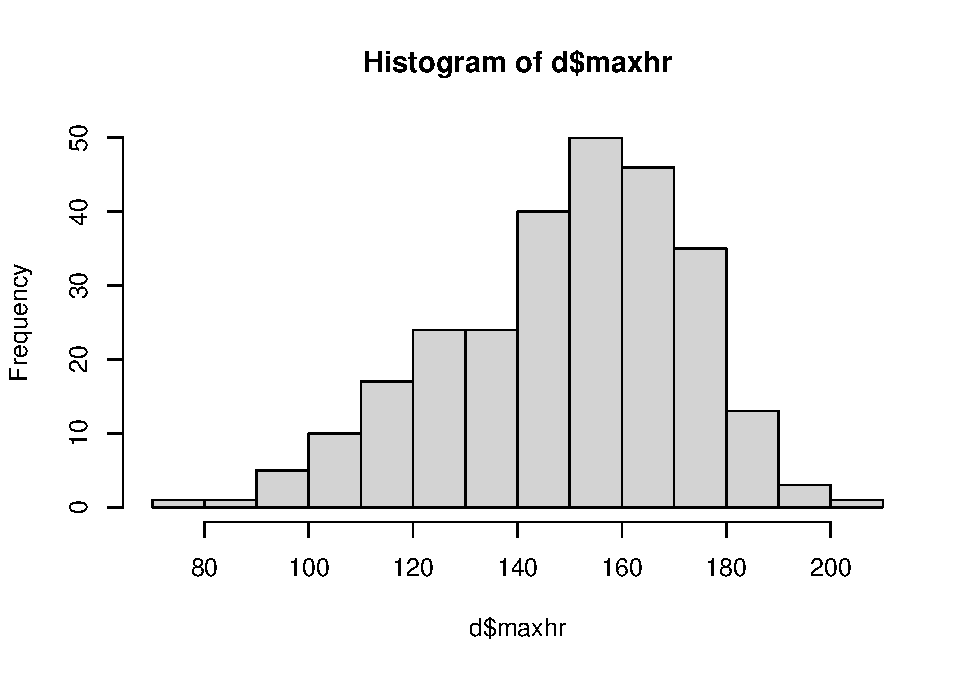
\includegraphics[width=0.8\linewidth]{heart_disease_ms_files/figure-latex/eda_x-3} \end{center}

\begin{Shaded}
\begin{Highlighting}[]
\FunctionTok{boxplot}\NormalTok{(maxhr }\SpecialCharTok{\textasciitilde{}}\NormalTok{ disease\_fct, d, }\AttributeTok{horizontal =} \ConstantTok{TRUE}\NormalTok{) }\CommentTok{\#good power of prediction }
\end{Highlighting}
\end{Shaded}

\begin{center}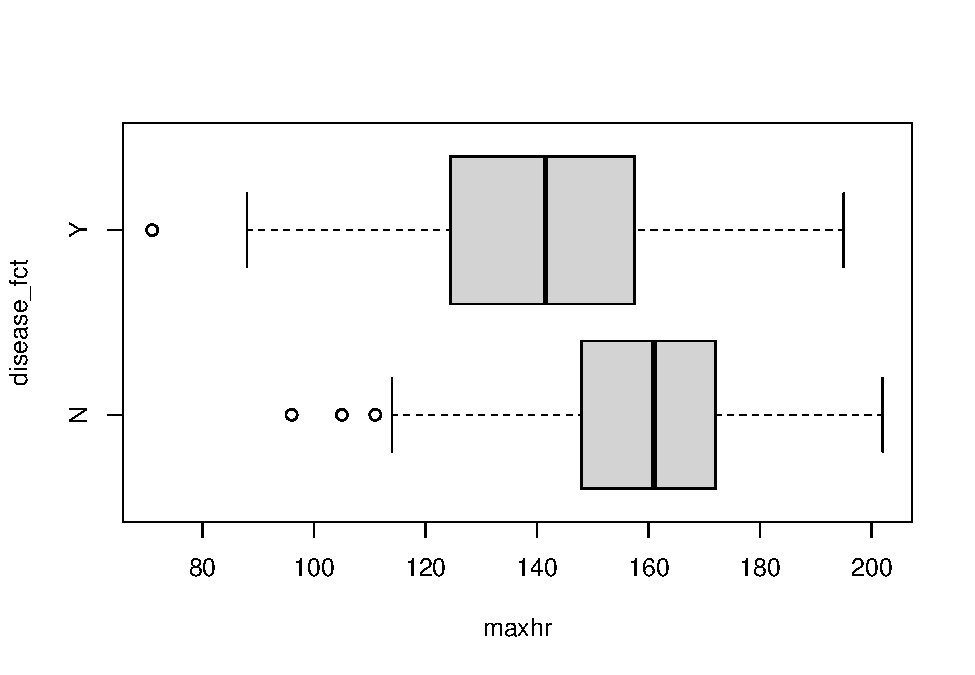
\includegraphics[width=0.8\linewidth]{heart_disease_ms_files/figure-latex/eda_x-4} \end{center}

\begin{Shaded}
\begin{Highlighting}[]
\NormalTok{d }\SpecialCharTok{\%\textgreater{}\%}
  \FunctionTok{group\_by}\NormalTok{(disease\_fct) }\SpecialCharTok{\%\textgreater{}\%}
  \FunctionTok{summarise}\NormalTok{(}\AttributeTok{median =} \FunctionTok{median}\NormalTok{(maxhr),}
            \AttributeTok{p25 =} \FunctionTok{quantile}\NormalTok{(maxhr, }\AttributeTok{p =} \FloatTok{0.25}\NormalTok{),}
            \AttributeTok{p75 =} \FunctionTok{quantile}\NormalTok{(maxhr, }\AttributeTok{p =} \FloatTok{0.75}\NormalTok{)) }
\end{Highlighting}
\end{Shaded}

\begin{verbatim}
## # A tibble: 2 x 4
##   disease_fct median   p25   p75
##   <fct>        <dbl> <dbl> <dbl>
## 1 N             161   148.  172 
## 2 Y             142.  125.  157.
\end{verbatim}

\begin{Shaded}
\begin{Highlighting}[]
\CommentTok{\#$ blood   \textless{}dbl\textgreater{} 130, 115, 124, 128, 120, 120, 130, 110, 140, 150, 135, 142, …}
\CommentTok{\# resting\_blood\_pressure (type: int): resting blood pressure}
\FunctionTok{get\_percentiles}\NormalTok{(d}\SpecialCharTok{$}\NormalTok{blood) }\CommentTok{\#94 to 200}
\end{Highlighting}
\end{Shaded}

\begin{verbatim}
##    0%    1%    5%   10%   25%   50%   75%   90%   95%   99%  100% 
##  94.0 100.0 106.9 110.0 120.0 130.0 140.0 152.0 160.0 180.0 200.0
\end{verbatim}

\begin{Shaded}
\begin{Highlighting}[]
\FunctionTok{hist}\NormalTok{(d}\SpecialCharTok{$}\NormalTok{blood) }\CommentTok{\#normalise but could cap at right}
\end{Highlighting}
\end{Shaded}

\begin{center}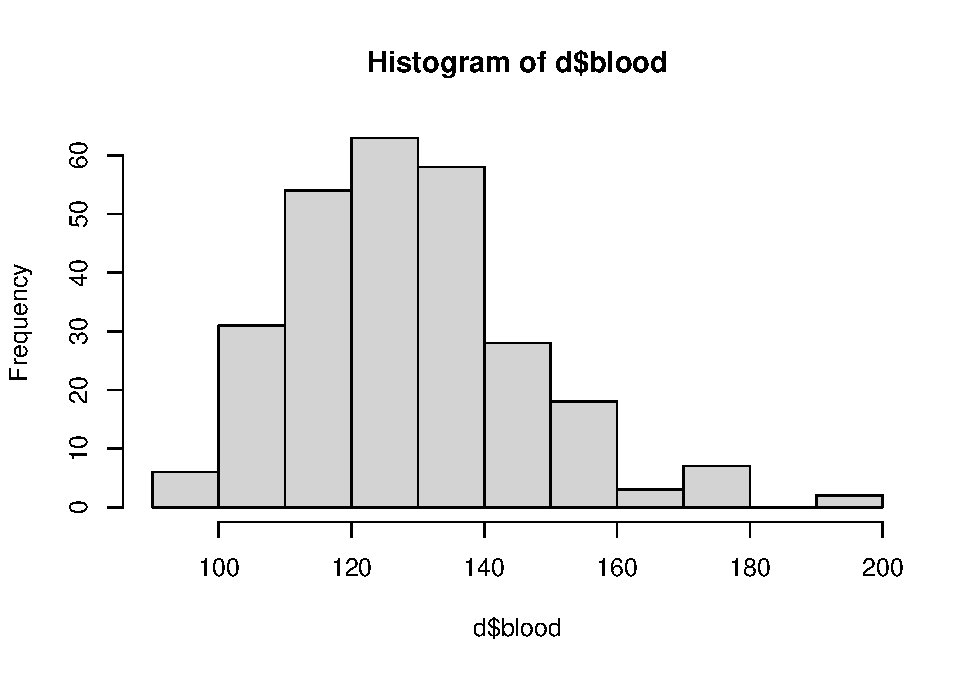
\includegraphics[width=0.8\linewidth]{heart_disease_ms_files/figure-latex/eda_x-5} \end{center}

\begin{Shaded}
\begin{Highlighting}[]
\FunctionTok{boxplot}\NormalTok{(blood }\SpecialCharTok{\textasciitilde{}}\NormalTok{ disease\_fct, d, }\AttributeTok{horizontal =} \ConstantTok{TRUE}\NormalTok{) }\CommentTok{\#no power of prediction }
\end{Highlighting}
\end{Shaded}

\begin{center}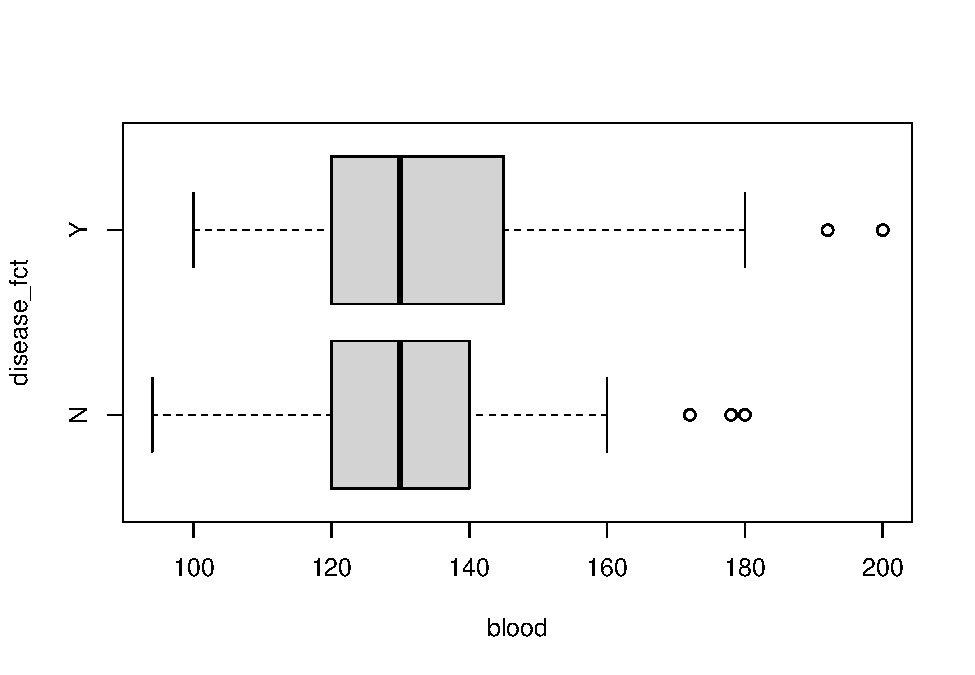
\includegraphics[width=0.8\linewidth]{heart_disease_ms_files/figure-latex/eda_x-6} \end{center}

\begin{Shaded}
\begin{Highlighting}[]
\NormalTok{d }\SpecialCharTok{\%\textgreater{}\%}
  \FunctionTok{group\_by}\NormalTok{(disease\_fct) }\SpecialCharTok{\%\textgreater{}\%}
  \FunctionTok{summarise}\NormalTok{(}\AttributeTok{median =} \FunctionTok{median}\NormalTok{(blood),}
            \AttributeTok{p25 =} \FunctionTok{quantile}\NormalTok{(blood, }\AttributeTok{p =} \FloatTok{0.25}\NormalTok{),}
            \AttributeTok{p75 =} \FunctionTok{quantile}\NormalTok{(blood, }\AttributeTok{p =} \FloatTok{0.75}\NormalTok{)) }\CommentTok{\#no power, but will leave}
\end{Highlighting}
\end{Shaded}

\begin{verbatim}
## # A tibble: 2 x 4
##   disease_fct median   p25   p75
##   <fct>        <dbl> <dbl> <dbl>
## 1 N              130   120   140
## 2 Y              130   120   145
\end{verbatim}

\begin{Shaded}
\begin{Highlighting}[]
\CommentTok{\# $ chol    \textless{}dbl\textgreater{} 322, 564, 261, 263, 269, 177, 256, 239, 293, 407, 234, 226, 235, 234, 303, 149, 3…}
\CommentTok{\# serum\_cholesterol\_mg\_per\_dl (type: int): serum cholestoral in mg/dl}
\FunctionTok{get\_percentiles}\NormalTok{(d}\SpecialCharTok{$}\NormalTok{chol) }\CommentTok{\#126 to 564}
\end{Highlighting}
\end{Shaded}

\begin{verbatim}
##     0%     1%     5%    10%    25%    50%    75%    90%    95%    99%   100% 
## 126.00 149.00 177.00 194.80 213.00 245.00 280.00 309.00 326.55 407.62 564.00
\end{verbatim}

\begin{Shaded}
\begin{Highlighting}[]
\FunctionTok{hist}\NormalTok{(d}\SpecialCharTok{$}\NormalTok{chol) }\CommentTok{\#normalise but could cap at right, but log is better}
\end{Highlighting}
\end{Shaded}

\begin{center}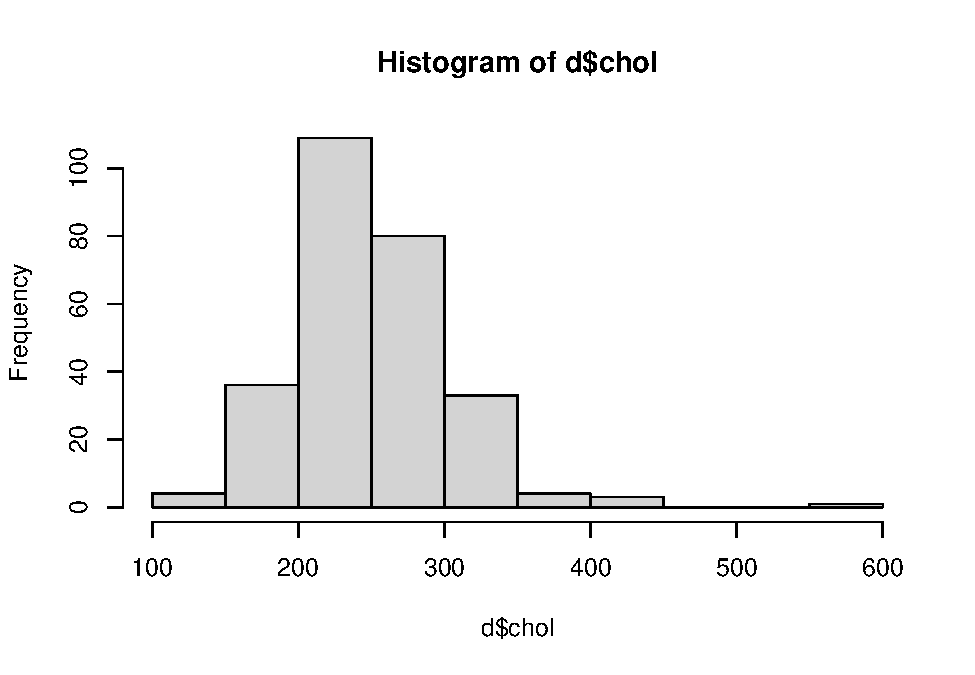
\includegraphics[width=0.8\linewidth]{heart_disease_ms_files/figure-latex/eda_x-7} \end{center}

\begin{Shaded}
\begin{Highlighting}[]
\FunctionTok{boxplot}\NormalTok{(chol }\SpecialCharTok{\textasciitilde{}}\NormalTok{ disease\_fct, d, }\AttributeTok{horizontal =} \ConstantTok{TRUE}\NormalTok{) }\CommentTok{\#some power}
\end{Highlighting}
\end{Shaded}

\begin{center}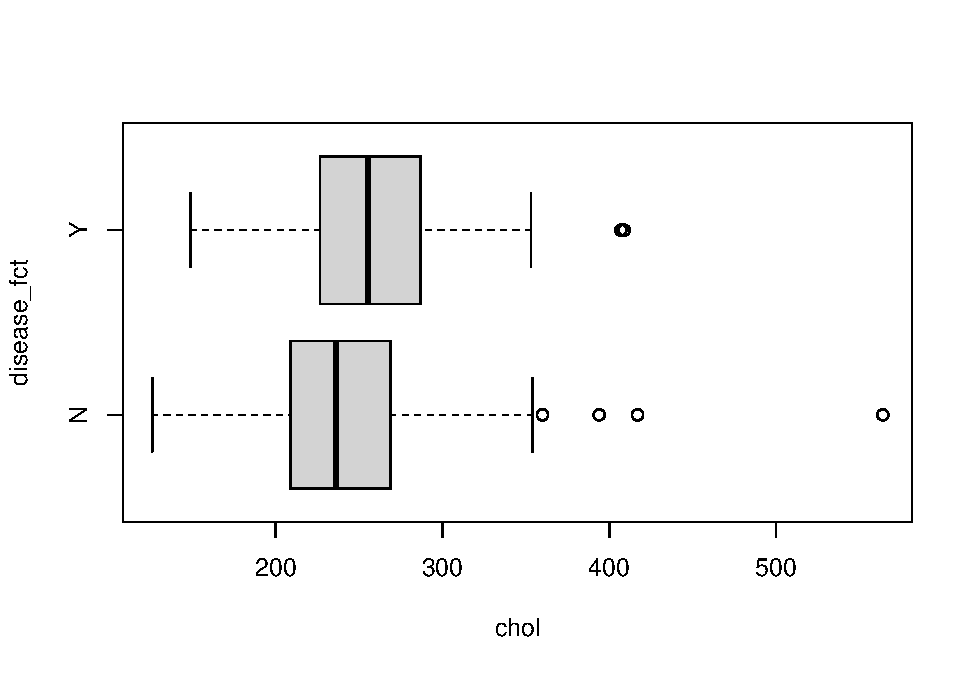
\includegraphics[width=0.8\linewidth]{heart_disease_ms_files/figure-latex/eda_x-8} \end{center}

\begin{Shaded}
\begin{Highlighting}[]
\NormalTok{d}\SpecialCharTok{$}\NormalTok{chol\_log }\OtherTok{\textless{}{-}} \FunctionTok{log}\NormalTok{(d}\SpecialCharTok{$}\NormalTok{chol)}

\FunctionTok{boxplot}\NormalTok{(chol\_log }\SpecialCharTok{\textasciitilde{}}\NormalTok{ disease\_fct, d, }\AttributeTok{horizontal =} \ConstantTok{TRUE}\NormalTok{) }\CommentTok{\#some power}
\end{Highlighting}
\end{Shaded}

\begin{center}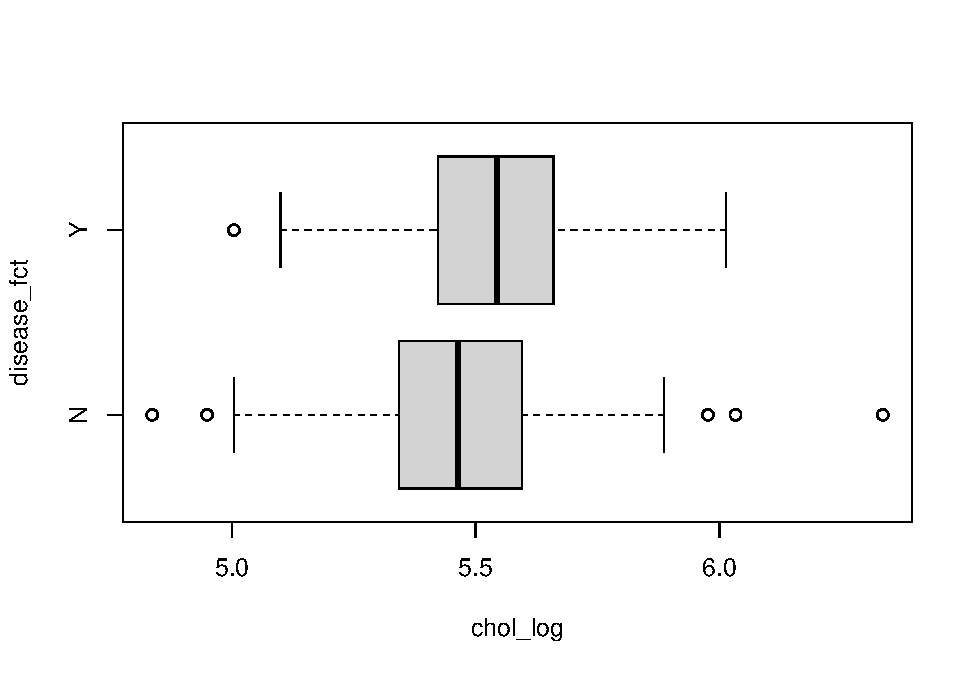
\includegraphics[width=0.8\linewidth]{heart_disease_ms_files/figure-latex/eda_x-9} \end{center}

\begin{Shaded}
\begin{Highlighting}[]
\NormalTok{d }\SpecialCharTok{\%\textgreater{}\%}
  \FunctionTok{group\_by}\NormalTok{(disease\_fct) }\SpecialCharTok{\%\textgreater{}\%}
  \FunctionTok{summarise}\NormalTok{(}\AttributeTok{median =} \FunctionTok{median}\NormalTok{(chol),}
            \AttributeTok{p25 =} \FunctionTok{quantile}\NormalTok{(chol, }\AttributeTok{p =} \FloatTok{0.25}\NormalTok{),}
            \AttributeTok{p75 =} \FunctionTok{quantile}\NormalTok{(chol, }\AttributeTok{p =} \FloatTok{0.75}\NormalTok{)) }\CommentTok{\#some power}
\end{Highlighting}
\end{Shaded}

\begin{verbatim}
## # A tibble: 2 x 4
##   disease_fct median   p25   p75
##   <fct>        <dbl> <dbl> <dbl>
## 1 N             236   209   269.
## 2 Y             256.  227.  286.
\end{verbatim}

\begin{Shaded}
\begin{Highlighting}[]
\CommentTok{\# $ oldpeak \textless{}dbl\textgreater{} 2.4, 1.6, 0.3, 0.2, 0.2, 0.4, 0.6, 1.2, 1.2, 4.0, 0.5, 0.0, …}
\CommentTok{\# ST depression induced by exercise relto rest, measure of abnormality in eco}
\FunctionTok{get\_percentiles}\NormalTok{(d}\SpecialCharTok{$}\NormalTok{oldpeak) }\CommentTok{\#mostly 0s from 0 to 6.2}
\end{Highlighting}
\end{Shaded}

\begin{verbatim}
##   0%   1%   5%  10%  25%  50%  75%  90%  95%  99% 100% 
## 0.00 0.00 0.00 0.00 0.00 0.80 1.60 2.60 3.31 4.20 6.20
\end{verbatim}

\begin{Shaded}
\begin{Highlighting}[]
\FunctionTok{hist}\NormalTok{(d}\SpecialCharTok{$}\NormalTok{oldpeak) }\CommentTok{\#skew to zero, no way to normalize}
\end{Highlighting}
\end{Shaded}

\begin{center}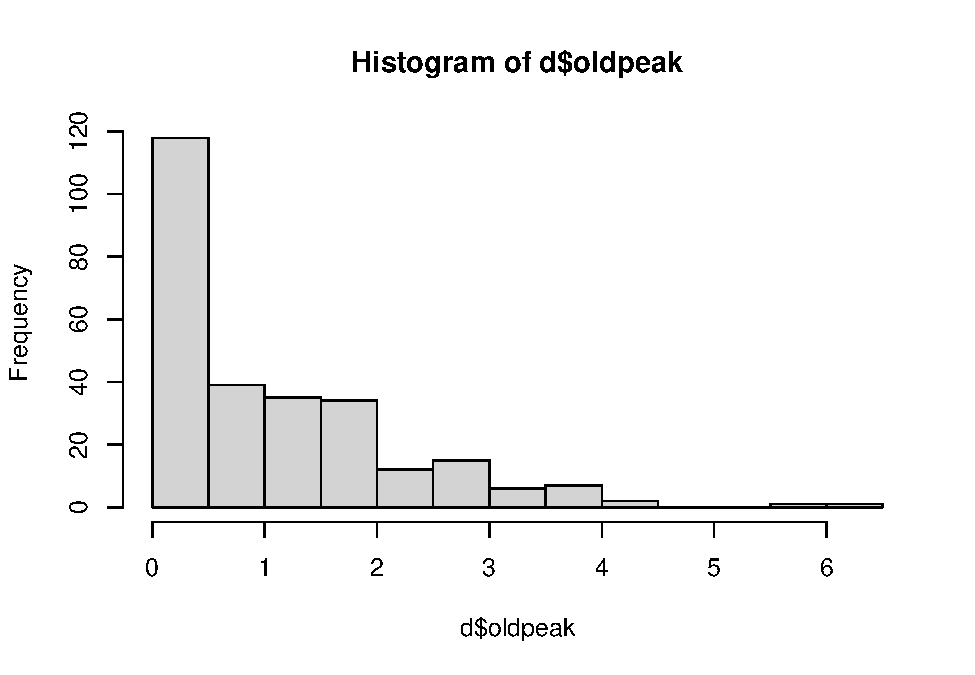
\includegraphics[width=0.8\linewidth]{heart_disease_ms_files/figure-latex/eda_x-10} \end{center}

\begin{Shaded}
\begin{Highlighting}[]
\FunctionTok{boxplot}\NormalTok{(oldpeak }\SpecialCharTok{\textasciitilde{}}\NormalTok{ disease\_fct, d, }\AttributeTok{horizontal =} \ConstantTok{TRUE}\NormalTok{) }\CommentTok{\#strong power}
\end{Highlighting}
\end{Shaded}

\begin{center}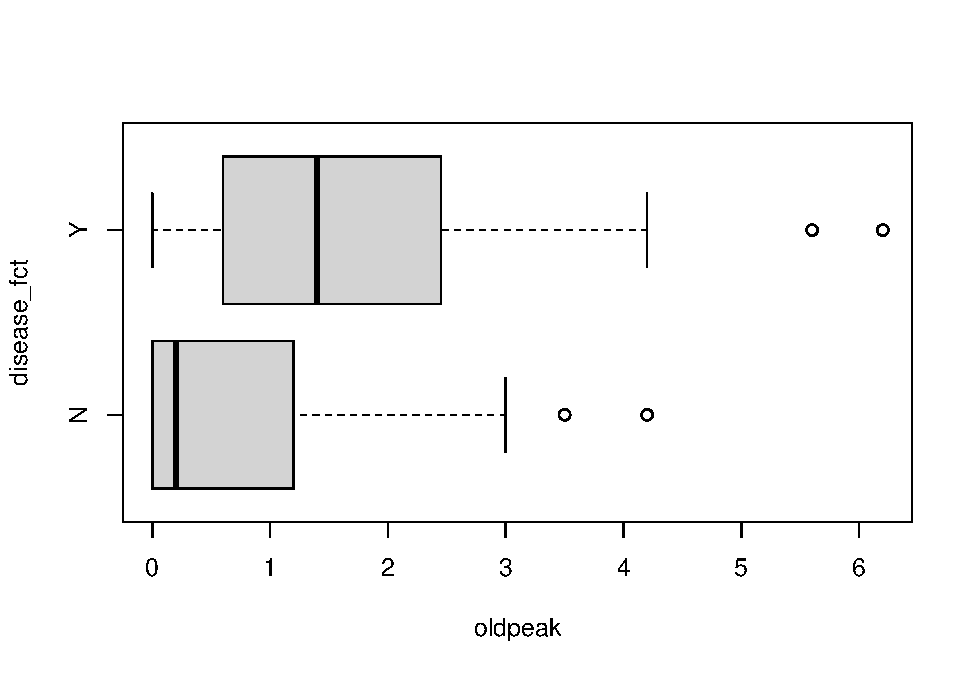
\includegraphics[width=0.8\linewidth]{heart_disease_ms_files/figure-latex/eda_x-11} \end{center}

\begin{Shaded}
\begin{Highlighting}[]
\NormalTok{d }\SpecialCharTok{\%\textgreater{}\%}
  \FunctionTok{group\_by}\NormalTok{(disease\_fct) }\SpecialCharTok{\%\textgreater{}\%}
  \FunctionTok{summarise}\NormalTok{(}\AttributeTok{median =} \FunctionTok{median}\NormalTok{(oldpeak),}
            \AttributeTok{p25 =} \FunctionTok{quantile}\NormalTok{(oldpeak, }\AttributeTok{p =} \FloatTok{0.25}\NormalTok{),}
            \AttributeTok{p75 =} \FunctionTok{quantile}\NormalTok{(oldpeak, }\AttributeTok{p =} \FloatTok{0.75}\NormalTok{)) }\CommentTok{\#has power}
\end{Highlighting}
\end{Shaded}

\begin{verbatim}
## # A tibble: 2 x 4
##   disease_fct median   p25   p75
##   <fct>        <dbl> <dbl> <dbl>
## 1 N              0.2   0    1.17
## 2 Y              1.4   0.6  2.42
\end{verbatim}

\begin{Shaded}
\begin{Highlighting}[]
\CommentTok{\# add a few discrete vars by cutting to test it out as well}
\NormalTok{d}\SpecialCharTok{$}\NormalTok{oldpeak\_flag }\OtherTok{=} \FunctionTok{as.factor}\NormalTok{(}\FunctionTok{ifelse}\NormalTok{(d}\SpecialCharTok{$}\NormalTok{oldpeak }\SpecialCharTok{==} \DecValTok{0}\NormalTok{, }\DecValTok{0}\NormalTok{, }\DecValTok{1}\NormalTok{))}

\NormalTok{(t }\OtherTok{\textless{}{-}} \FunctionTok{table}\NormalTok{(d}\SpecialCharTok{$}\NormalTok{oldpeak\_flag, d}\SpecialCharTok{$}\NormalTok{disease\_fct))}
\end{Highlighting}
\end{Shaded}

\begin{verbatim}
##    
##      N  Y
##   0 63 22
##   1 87 98
\end{verbatim}

\begin{Shaded}
\begin{Highlighting}[]
\FunctionTok{round}\NormalTok{(}\FunctionTok{prop.table}\NormalTok{(t, }\AttributeTok{margin =} \DecValTok{2}\NormalTok{), }\DecValTok{2}\NormalTok{) }\CommentTok{\# good power }
\end{Highlighting}
\end{Shaded}

\begin{verbatim}
##    
##        N    Y
##   0 0.42 0.18
##   1 0.58 0.82
\end{verbatim}

\begin{Shaded}
\begin{Highlighting}[]
\NormalTok{m }\OtherTok{\textless{}{-}}\NormalTok{ d }\CommentTok{\# modeling dataset}

\CommentTok{\# remove vars that were modified for modeling}
\NormalTok{m }\OtherTok{\textless{}{-}}\NormalTok{ m }\SpecialCharTok{\%\textgreater{}\%}
  \FunctionTok{select}\NormalTok{(}\SpecialCharTok{{-}}\NormalTok{sex, }\SpecialCharTok{{-}}\NormalTok{pain, }\SpecialCharTok{{-}}\NormalTok{sugar, }\SpecialCharTok{{-}}\NormalTok{electro, }\SpecialCharTok{{-}}\NormalTok{angina, }\SpecialCharTok{{-}}\NormalTok{vessels, }\SpecialCharTok{{-}}\NormalTok{slope, }\SpecialCharTok{{-}}\NormalTok{chol,}
         \SpecialCharTok{{-}}\NormalTok{thal)}

\CommentTok{\# split into training and testing}
\FunctionTok{set.seed}\NormalTok{(}\DecValTok{23489}\NormalTok{)}
\NormalTok{train\_index }\OtherTok{\textless{}{-}} \FunctionTok{sample}\NormalTok{(}\DecValTok{1}\SpecialCharTok{:}\FunctionTok{nrow}\NormalTok{(m), }\FloatTok{0.8} \SpecialCharTok{*} \FunctionTok{nrow}\NormalTok{(m))}
\NormalTok{m\_train }\OtherTok{\textless{}{-}}\NormalTok{ m[train\_index, ]}
\NormalTok{m\_test }\OtherTok{\textless{}{-}}\NormalTok{ m[}\SpecialCharTok{{-}}\NormalTok{train\_index, ]}
\end{Highlighting}
\end{Shaded}

\begin{Shaded}
\begin{Highlighting}[]
\CommentTok{\# fit a random forest model }
\NormalTok{rf\_fit }\OtherTok{\textless{}{-}} \FunctionTok{train}\NormalTok{(disease\_fct }\SpecialCharTok{\textasciitilde{}}\NormalTok{ . }\SpecialCharTok{{-}}\NormalTok{ oldpeak\_flag, }
                \AttributeTok{data =}\NormalTok{ m\_train, }
                \AttributeTok{method =} \StringTok{"rf"}\NormalTok{,}
                \AttributeTok{importance =} \ConstantTok{TRUE}\NormalTok{)}

\NormalTok{rf\_fit}
\end{Highlighting}
\end{Shaded}

\begin{verbatim}
## Random Forest 
## 
## 216 samples
##  14 predictor
##   2 classes: 'N', 'Y' 
## 
## No pre-processing
## Resampling: Bootstrapped (25 reps) 
## Summary of sample sizes: 216, 216, 216, 216, 216, 216, ... 
## Resampling results across tuning parameters:
## 
##   mtry  Accuracy   Kappa    
##    2    0.7982270  0.5942971
##    7    0.7723457  0.5417662
##   13    0.7609714  0.5196511
## 
## Accuracy was used to select the optimal model using the largest value.
## The final value used for the model was mtry = 2.
\end{verbatim}

\begin{Shaded}
\begin{Highlighting}[]
\CommentTok{\# predict the outcome on a test set and assess accuracy of model}
\NormalTok{m\_rf\_pred }\OtherTok{\textless{}{-}} \FunctionTok{predict}\NormalTok{(rf\_fit, m\_test)}

\FunctionTok{confusionMatrix}\NormalTok{(m\_rf\_pred, m\_test}\SpecialCharTok{$}\NormalTok{disease\_fct) }\CommentTok{\#85\% acc}
\end{Highlighting}
\end{Shaded}

\begin{verbatim}
## Confusion Matrix and Statistics
## 
##           Reference
## Prediction  N  Y
##          N 32  5
##          Y  3 14
##                                           
##                Accuracy : 0.8519          
##                  95% CI : (0.7288, 0.9338)
##     No Information Rate : 0.6481          
##     P-Value [Acc > NIR] : 0.0007545       
##                                           
##                   Kappa : 0.6672          
##                                           
##  Mcnemar's Test P-Value : 0.7236736       
##                                           
##             Sensitivity : 0.9143          
##             Specificity : 0.7368          
##          Pos Pred Value : 0.8649          
##          Neg Pred Value : 0.8235          
##              Prevalence : 0.6481          
##          Detection Rate : 0.5926          
##    Detection Prevalence : 0.6852          
##       Balanced Accuracy : 0.8256          
##                                           
##        'Positive' Class : N               
## 
\end{verbatim}

\begin{Shaded}
\begin{Highlighting}[]
\CommentTok{\# plot important features}
\NormalTok{importance }\OtherTok{\textless{}{-}} \FunctionTok{varImp}\NormalTok{(rf\_fit, }\AttributeTok{scale =} \ConstantTok{FALSE}\NormalTok{)}
\FunctionTok{plot}\NormalTok{(importance)}
\end{Highlighting}
\end{Shaded}

\begin{center}\includegraphics[width=0.8\linewidth]{heart_disease_ms_files/figure-latex/ml_rf_caret-1} \end{center}

\begin{Shaded}
\begin{Highlighting}[]
\NormalTok{importance\_df }\OtherTok{\textless{}{-}}\NormalTok{ importance}\SpecialCharTok{$}\NormalTok{importance}
\NormalTok{importance\_df}\SpecialCharTok{$}\NormalTok{feature }\OtherTok{\textless{}{-}} \FunctionTok{rownames}\NormalTok{(importance\_df)}

\FunctionTok{ggplot}\NormalTok{(importance\_df, }\FunctionTok{aes}\NormalTok{(}\FunctionTok{reorder}\NormalTok{(feature, }\SpecialCharTok{+}\NormalTok{N), N)) }\SpecialCharTok{+}
  \FunctionTok{geom\_col}\NormalTok{() }\SpecialCharTok{+}
  \FunctionTok{coord\_flip}\NormalTok{()}
\end{Highlighting}
\end{Shaded}

\begin{center}\includegraphics[width=0.8\linewidth]{heart_disease_ms_files/figure-latex/ml_rf_caret-2} \end{center}

\begin{Shaded}
\begin{Highlighting}[]
\CommentTok{\# Forward subset selection}
\NormalTok{reg0 }\OtherTok{\textless{}{-}} \FunctionTok{glm}\NormalTok{(disease\_fct }\SpecialCharTok{\textasciitilde{}} \DecValTok{1}\NormalTok{, }\AttributeTok{data =}\NormalTok{ m\_train, }\AttributeTok{family =}\NormalTok{ binomial) }\CommentTok{\#base}
\NormalTok{reg1 }\OtherTok{\textless{}{-}} \FunctionTok{glm}\NormalTok{(disease\_fct }\SpecialCharTok{\textasciitilde{}}\NormalTok{ ., }\AttributeTok{data =}\NormalTok{ m\_train, }\AttributeTok{family =}\NormalTok{ binomial) }\CommentTok{\#full}
\FunctionTok{summary}\NormalTok{(reg1)}
\end{Highlighting}
\end{Shaded}

\begin{verbatim}
## 
## Call:
## glm(formula = disease_fct ~ ., family = binomial, data = m_train)
## 
## Coefficients:
##                     Estimate Std. Error z value Pr(>|z|)    
## (Intercept)        -10.80447    7.87706  -1.372 0.170176    
## age                 -0.01403    0.03172  -0.442 0.658287    
## blood                0.02830    0.01327   2.133 0.032946 *  
## maxhr               -0.04323    0.01434  -3.015 0.002569 ** 
## oldpeak              0.78295    0.30845   2.538 0.011139 *  
## sex_fctM             2.05918    0.65815   3.129 0.001756 ** 
## pain_fct4            1.71162    0.48024   3.564 0.000365 ***
## sugar_fctY           0.10400    0.63172   0.165 0.869238    
## electro_fct2         0.69031    0.47309   1.459 0.144519    
## angina_fctY          0.53931    0.52120   1.035 0.300794    
## vessels_fct2-3       1.63240    0.69266   2.357 0.018439 *  
## slope_fct2           1.13985    0.55952   2.037 0.041630 *  
## thal_fctreversable   1.75173    0.51068   3.430 0.000603 ***
## chol_log             1.85422    1.43280   1.294 0.195623    
## oldpeak_flag1       -1.72395    0.73844  -2.335 0.019565 *  
## ---
## Signif. codes:  0 '***' 0.001 '**' 0.01 '*' 0.05 '.' 0.1 ' ' 1
## 
## (Dispersion parameter for binomial family taken to be 1)
## 
##     Null deviance: 298.53  on 215  degrees of freedom
## Residual deviance: 134.80  on 201  degrees of freedom
## AIC: 164.8
## 
## Number of Fisher Scoring iterations: 6
\end{verbatim}

\begin{Shaded}
\begin{Highlighting}[]
\NormalTok{best }\OtherTok{\textless{}{-}} \FunctionTok{step}\NormalTok{(reg0, }\AttributeTok{scope =} \FunctionTok{formula}\NormalTok{(reg1), }
             \AttributeTok{direction =} \StringTok{"forward"}\NormalTok{, }\AttributeTok{k =} \DecValTok{2}\NormalTok{) }\CommentTok{\#k=2 is AIC, best}
\end{Highlighting}
\end{Shaded}

\begin{verbatim}
## Start:  AIC=300.53
## disease_fct ~ 1
## 
##                Df Deviance    AIC
## + pain_fct      1   240.09 244.09
## + thal_fct      1   244.73 248.73
## + maxhr         1   256.00 260.00
## + oldpeak       1   256.89 260.89
## + angina_fct    1   261.19 265.19
## + slope_fct     1   271.68 275.68
## + sex_fct       1   272.30 276.30
## + vessels_fct   1   277.88 281.88
## + oldpeak_flag  1   284.95 288.95
## + age           1   288.83 292.83
## + blood         1   290.99 294.99
## + electro_fct   1   294.77 298.77
## + chol_log      1   295.75 299.75
## <none>              298.53 300.53
## + sugar_fct     1   298.37 302.37
## 
## Step:  AIC=244.09
## disease_fct ~ pain_fct
## 
##                Df Deviance    AIC
## + thal_fct      1   208.07 214.07
## + oldpeak       1   209.89 215.89
## + maxhr         1   217.94 223.94
## + sex_fct       1   219.11 225.11
## + slope_fct     1   219.81 225.81
## + angina_fct    1   224.32 230.32
## + vessels_fct   1   228.65 234.65
## + oldpeak_flag  1   231.00 237.00
## + blood         1   232.21 238.21
## + age           1   233.54 239.54
## <none>              240.09 244.09
## + electro_fct   1   238.24 244.24
## + sugar_fct     1   238.55 244.55
## + chol_log      1   238.90 244.90
## 
## Step:  AIC=214.07
## disease_fct ~ pain_fct + thal_fct
## 
##                Df Deviance    AIC
## + oldpeak       1   185.10 193.10
## + maxhr         1   187.71 195.71
## + slope_fct     1   190.93 198.93
## + vessels_fct   1   197.15 205.15
## + angina_fct    1   198.29 206.29
## + sex_fct       1   199.74 207.74
## + age           1   200.83 208.83
## + blood         1   201.72 209.72
## + electro_fct   1   202.82 210.82
## + oldpeak_flag  1   204.05 212.05
## <none>              208.07 214.07
## + chol_log      1   206.46 214.46
## + sugar_fct     1   207.07 215.07
## 
## Step:  AIC=193.1
## disease_fct ~ pain_fct + thal_fct + oldpeak
## 
##                Df Deviance    AIC
## + maxhr         1   174.86 184.86
## + sex_fct       1   177.60 187.60
## + vessels_fct   1   178.48 188.48
## + angina_fct    1   179.04 189.04
## + slope_fct     1   179.37 189.37
## + electro_fct   1   180.82 190.82
## + age           1   181.48 191.48
## + blood         1   181.52 191.52
## + oldpeak_flag  1   182.87 192.87
## + chol_log      1   183.03 193.03
## <none>              185.10 193.10
## + sugar_fct     1   183.99 193.99
## 
## Step:  AIC=184.86
## disease_fct ~ pain_fct + thal_fct + oldpeak + maxhr
## 
##                Df Deviance    AIC
## + sex_fct       1   164.70 176.70
## + vessels_fct   1   169.22 181.22
## + blood         1   169.46 181.46
## + oldpeak_flag  1   169.88 181.88
## + electro_fct   1   171.05 183.05
## + angina_fct    1   171.17 183.17
## + slope_fct     1   171.96 183.96
## <none>              174.86 184.86
## + chol_log      1   172.86 184.86
## + sugar_fct     1   173.65 185.65
## + age           1   174.42 186.42
## 
## Step:  AIC=176.7
## disease_fct ~ pain_fct + thal_fct + oldpeak + maxhr + sex_fct
## 
##                Df Deviance    AIC
## + blood         1   155.75 169.75
## + vessels_fct   1   158.89 172.89
## + chol_log      1   159.77 173.77
## + oldpeak_flag  1   160.00 174.00
## + slope_fct     1   161.60 175.60
## + electro_fct   1   162.09 176.09
## + angina_fct    1   162.24 176.24
## <none>              164.70 176.70
## + age           1   163.48 177.48
## + sugar_fct     1   163.74 177.74
## 
## Step:  AIC=169.75
## disease_fct ~ pain_fct + thal_fct + oldpeak + maxhr + sex_fct + 
##     blood
## 
##                Df Deviance    AIC
## + vessels_fct   1   150.50 166.50
## + oldpeak_flag  1   151.94 167.94
## + chol_log      1   152.38 168.38
## + slope_fct     1   153.08 169.08
## + electro_fct   1   153.27 169.27
## <none>              155.75 169.75
## + angina_fct    1   154.18 170.18
## + sugar_fct     1   155.44 171.44
## + age           1   155.71 171.71
## 
## Step:  AIC=166.5
## disease_fct ~ pain_fct + thal_fct + oldpeak + maxhr + sex_fct + 
##     blood + vessels_fct
## 
##                Df Deviance    AIC
## + oldpeak_flag  1   146.69 164.69
## + chol_log      1   147.28 165.28
## + slope_fct     1   147.39 165.39
## + electro_fct   1   147.68 165.68
## + angina_fct    1   148.39 166.39
## <none>              150.50 166.50
## + age           1   150.34 168.34
## + sugar_fct     1   150.42 168.42
## 
## Step:  AIC=164.69
## disease_fct ~ pain_fct + thal_fct + oldpeak + maxhr + sex_fct + 
##     blood + vessels_fct + oldpeak_flag
## 
##               Df Deviance    AIC
## + slope_fct    1   140.21 160.21
## + chol_log     1   143.34 163.34
## + electro_fct  1   143.52 163.52
## <none>             146.69 164.69
## + angina_fct   1   145.19 165.19
## + sugar_fct    1   146.51 166.51
## + age          1   146.69 166.69
## 
## Step:  AIC=160.21
## disease_fct ~ pain_fct + thal_fct + oldpeak + maxhr + sex_fct + 
##     blood + vessels_fct + oldpeak_flag + slope_fct
## 
##               Df Deviance    AIC
## + electro_fct  1   137.76 159.76
## + chol_log     1   137.94 159.94
## <none>             140.21 160.21
## + angina_fct   1   139.29 161.29
## + sugar_fct    1   140.17 162.17
## + age          1   140.20 162.20
## 
## Step:  AIC=159.76
## disease_fct ~ pain_fct + thal_fct + oldpeak + maxhr + sex_fct + 
##     blood + vessels_fct + oldpeak_flag + slope_fct + electro_fct
## 
##              Df Deviance    AIC
## <none>            137.76 159.76
## + chol_log    1   136.03 160.03
## + angina_fct  1   136.66 160.66
## + sugar_fct   1   137.69 161.69
## + age         1   137.72 161.72
\end{verbatim}

\begin{Shaded}
\begin{Highlighting}[]
\FunctionTok{summary}\NormalTok{(best)}
\end{Highlighting}
\end{Shaded}

\begin{verbatim}
## 
## Call:
## glm(formula = disease_fct ~ pain_fct + thal_fct + oldpeak + maxhr + 
##     sex_fct + blood + vessels_fct + oldpeak_flag + slope_fct + 
##     electro_fct, family = binomial, data = m_train)
## 
## Coefficients:
##                    Estimate Std. Error z value Pr(>|z|)    
## (Intercept)        -1.82376    2.38999  -0.763 0.445414    
## pain_fct4           1.83861    0.45425   4.048 5.18e-05 ***
## thal_fctreversable  1.82962    0.50183   3.646 0.000266 ***
## oldpeak             0.81356    0.29593   2.749 0.005974 ** 
## maxhr              -0.04051    0.01226  -3.305 0.000950 ***
## sex_fctM            1.88806    0.60643   3.113 0.001849 ** 
## blood               0.03002    0.01219   2.462 0.013805 *  
## vessels_fct2-3      1.54362    0.64650   2.388 0.016957 *  
## oldpeak_flag1      -1.85117    0.71643  -2.584 0.009770 ** 
## slope_fct2          1.27240    0.54438   2.337 0.019422 *  
## electro_fct2        0.71193    0.46189   1.541 0.123238    
## ---
## Signif. codes:  0 '***' 0.001 '**' 0.01 '*' 0.05 '.' 0.1 ' ' 1
## 
## (Dispersion parameter for binomial family taken to be 1)
## 
##     Null deviance: 298.53  on 215  degrees of freedom
## Residual deviance: 137.76  on 205  degrees of freedom
## AIC: 159.76
## 
## Number of Fisher Scoring iterations: 6
\end{verbatim}

\begin{Shaded}
\begin{Highlighting}[]
\NormalTok{best}\SpecialCharTok{$}\NormalTok{anova}
\end{Highlighting}
\end{Shaded}

\begin{verbatim}
##              Step Df  Deviance Resid. Df Resid. Dev      AIC
## 1                 NA        NA       215   298.5315 300.5315
## 2      + pain_fct -1 58.441208       214   240.0903 244.0903
## 3      + thal_fct -1 32.018313       213   208.0720 214.0720
## 4       + oldpeak -1 22.973652       212   185.0984 193.0984
## 5         + maxhr -1 10.242545       211   174.8558 184.8558
## 6       + sex_fct -1 10.156776       210   164.6990 176.6990
## 7         + blood -1  8.948519       209   155.7505 169.7505
## 8   + vessels_fct -1  5.249137       208   150.5014 166.5014
## 9  + oldpeak_flag -1  3.806976       207   146.6944 164.6944
## 10    + slope_fct -1  6.481673       206   140.2127 160.2127
## 11  + electro_fct -1  2.453166       205   137.7596 159.7596
\end{verbatim}

\begin{Shaded}
\begin{Highlighting}[]
\CommentTok{\# predict the outcome on a test set and assess accuracy of model}
\NormalTok{m\_glm\_pred }\OtherTok{\textless{}{-}} \FunctionTok{predict}\NormalTok{(best, m\_test, }\AttributeTok{type =} \StringTok{"response"}\NormalTok{)}
\NormalTok{m\_glm\_pred }\OtherTok{\textless{}{-}} \FunctionTok{as.factor}\NormalTok{(}\FunctionTok{ifelse}\NormalTok{(m\_glm\_pred }\SpecialCharTok{\textgreater{}} \FloatTok{0.5}\NormalTok{, }\StringTok{"Y"}\NormalTok{, }\StringTok{"N"}\NormalTok{))}

\FunctionTok{confusionMatrix}\NormalTok{(m\_glm\_pred, m\_test}\SpecialCharTok{$}\NormalTok{disease\_fct) }\CommentTok{\#83\% acc}
\end{Highlighting}
\end{Shaded}

\begin{verbatim}
## Confusion Matrix and Statistics
## 
##           Reference
## Prediction  N  Y
##          N 31  5
##          Y  4 14
##                                           
##                Accuracy : 0.8333          
##                  95% CI : (0.7071, 0.9208)
##     No Information Rate : 0.6481          
##     P-Value [Acc > NIR] : 0.002228        
##                                           
##                   Kappa : 0.6301          
##                                           
##  Mcnemar's Test P-Value : 1.000000        
##                                           
##             Sensitivity : 0.8857          
##             Specificity : 0.7368          
##          Pos Pred Value : 0.8611          
##          Neg Pred Value : 0.7778          
##              Prevalence : 0.6481          
##          Detection Rate : 0.5741          
##    Detection Prevalence : 0.6667          
##       Balanced Accuracy : 0.8113          
##                                           
##        'Positive' Class : N               
## 
\end{verbatim}

\begin{Shaded}
\begin{Highlighting}[]
\CommentTok{\# A fancier rf model with gride search to see if accuracy improves}

\CommentTok{\# 10 folds and keep 3 folds for training. search method is grid.}
\NormalTok{control }\OtherTok{\textless{}{-}} \FunctionTok{trainControl}\NormalTok{(}\CommentTok{\#method=\textquotesingle{}repeatedcv\textquotesingle{}, }
                        \AttributeTok{method =} \StringTok{\textquotesingle{}cv\textquotesingle{}}\NormalTok{,}
                        \AttributeTok{number=}\DecValTok{10}\NormalTok{, }
                        \CommentTok{\#repeats=3, }
                        \AttributeTok{search=}\StringTok{\textquotesingle{}grid\textquotesingle{}}\NormalTok{)}

\CommentTok{\# Create tunegrid with 10 values for mtry to tunning model}
\NormalTok{tunegrid }\OtherTok{\textless{}{-}} \FunctionTok{expand.grid}\NormalTok{(}\AttributeTok{.mtry =}\NormalTok{ (}\DecValTok{1}\SpecialCharTok{:}\DecValTok{10}\NormalTok{)) }

\NormalTok{rf\_gridsearch }\OtherTok{\textless{}{-}} \FunctionTok{train}\NormalTok{(disease\_fct }\SpecialCharTok{\textasciitilde{}}\NormalTok{ ., }
                       \AttributeTok{data =}\NormalTok{ m,}
                       \AttributeTok{method =} \StringTok{\textquotesingle{}rf\textquotesingle{}}\NormalTok{,}
                       \AttributeTok{metric =} \StringTok{\textquotesingle{}Accuracy\textquotesingle{}}\NormalTok{,}
                       \AttributeTok{tuneGrid =}\NormalTok{ tunegrid,}
                       \AttributeTok{trControl =}\NormalTok{ control,}
                       \AttributeTok{importance =} \ConstantTok{TRUE}\NormalTok{)}

\FunctionTok{print}\NormalTok{(rf\_gridsearch) }\CommentTok{\#81\% acc}
\end{Highlighting}
\end{Shaded}

\begin{verbatim}
## Random Forest 
## 
## 270 samples
##  14 predictor
##   2 classes: 'N', 'Y' 
## 
## No pre-processing
## Resampling: Cross-Validated (10 fold) 
## Summary of sample sizes: 243, 243, 243, 243, 243, 243, ... 
## Resampling results across tuning parameters:
## 
##   mtry  Accuracy   Kappa    
##    1    0.8000000  0.5880798
##    2    0.7962963  0.5841140
##    3    0.7851852  0.5612804
##    4    0.7851852  0.5618665
##    5    0.7925926  0.5770145
##    6    0.7851852  0.5618651
##    7    0.7814815  0.5540500
##    8    0.7777778  0.5460016
##    9    0.7777778  0.5475338
##   10    0.7666667  0.5234864
## 
## Accuracy was used to select the optimal model using the largest value.
## The final value used for the model was mtry = 1.
\end{verbatim}

\begin{Shaded}
\begin{Highlighting}[]
\NormalTok{t }\OtherTok{\textless{}{-}} \FunctionTok{table}\NormalTok{(d}\SpecialCharTok{$}\NormalTok{disease\_fct, d}\SpecialCharTok{$}\NormalTok{thal\_fct)}
\NormalTok{p }\OtherTok{\textless{}{-}} \FunctionTok{prop.table}\NormalTok{(t,}\DecValTok{2}\NormalTok{)}
\FunctionTok{row.names}\NormalTok{(p) }\OtherTok{\textless{}{-}} \FunctionTok{c}\NormalTok{(}\StringTok{"No"}\NormalTok{, }\StringTok{"Yes"}\NormalTok{)}
\NormalTok{column\_names\_p }\OtherTok{\textless{}{-}} \FunctionTok{c}\NormalTok{(}\StringTok{"Normal or Fixed"}\NormalTok{, }\StringTok{"Reversable"}\NormalTok{)}

\FunctionTok{kable}\NormalTok{(p,}
      \AttributeTok{row.names =} \ConstantTok{TRUE}\NormalTok{,}
      \AttributeTok{col.names =}\NormalTok{ column\_names\_p,}
      \AttributeTok{digits =} \DecValTok{2}\NormalTok{,}
      \AttributeTok{caption =} \StringTok{"Thal \% of sick"}\NormalTok{,}
      \AttributeTok{booktabs =}\NormalTok{ T,}
      \AttributeTok{linesep =} \StringTok{""}
      \CommentTok{\#format = "latex"}
\NormalTok{) }\SpecialCharTok{\%\textgreater{}\%}
\FunctionTok{kable\_styling}\NormalTok{(}\AttributeTok{latex\_options =} \FunctionTok{c}\NormalTok{(}\StringTok{"striped"}\NormalTok{, }\StringTok{"hold\_position"}\NormalTok{))}
\end{Highlighting}
\end{Shaded}

\begin{longtable}[t]{lrr}
\caption{\label{tab:unnamed-chunk-1}Thal % of sick}\\
\toprule
 & Normal or Fixed & Reversable\\
\midrule
\cellcolor{gray!10}{No} & \cellcolor{gray!10}{0.75} & \cellcolor{gray!10}{0.24}\\
Yes & 0.25 & 0.76\\
\bottomrule
\end{longtable}

\#multi colinearity

\subsection{Intro}\label{intro}

270 x 14

plot pain, thal, hr, sex, oldpeak, angina, slope, vessels, blood\ldots.
not important chol, sugar

\section{References}\label{references}

\url{https://rebeccabarter.com/blog/2020-03-25_machine_learning}
\url{https://www.youtube.com/watch?v=OYWnuiPbmJQ}

\#rtree \#mdl1\_tree \textless- rpart(disease\_fct \textasciitilde{} .,
m\_train) \#mdl1\_tree \#plot(mdl1\_tree) \#text(mdl1\_tree)

\#3mdl1\_rf \textless- randomForest(disease\_fct \textasciitilde{} . -
oldpeak\_flag , \# data = m, \# importance = TRUE) \#summary(mdl1\_rf)
\#varImpPlot(mdl1\_rf) \#importance\_vars\_acc \textless-
varImpPlot(mdl1\_rf){[},1{]} \#df \textless-
data.frame(names(importance\_vars\_acc), \# importance\_vars\_acc)
\#colnames(df) \textless- c(``feature'', ``value'') \#df

vars \textless- c() ``age'' = ``Age'' ``blood'' = ``Fasting blood sugar
\textgreater{} 120 mg/dl'' ``maxhr'' ``oldpeak'' ``sex\_fct''
``pain\_fct'' ``sugar\_fct'' ``electro\_fct'' ``angina\_fct''
``vessels\_fct''

h \textless- hash(``age'' = ``Age'', ``blood'' = ``Fasting blood sugar
\textgreater{} 120 mg/dl'' ) h h{[}{[}``blood''{]}{]}

h \textless- hash() h \textless- hash( a=1, b=2, c=3 ) var \textless-
c(``vara'', ``varb'') nam \textless- c(``a largo'', ``b hombre'') h
\textless- hash(var, nam) h h{[}{[}``vara''{]}{]}

\end{document}
